\subsection{《1491:前哥伦布时代美洲启示录》}

标签: 世界历史 \ 美洲史

英文书名:1491: New Revelations of the Americas before Columbus

作者:【美】查尔斯·曼恩(Charles C. Mann)


\subsubsection{标注}
1. 1492年以前的西半球,按照当时的观点,这是一个欣欣向荣的、惊人地
多元的地方,语言、贸易、文化纷杂混乱;上千万人在这里爱着、恨着、
崇拜着,就像人们到处都在做的一样。在哥伦布之后,这个世界的大部分
都消失了,被病毒和镇压清空了。这种抹杀是如此之彻底,以至于在几代
人的时间里,征服者和被征服者都无从得知这个世界曾经存在了。

2. 印第安人并不全是不幸的受害者。多数奴隶都是战俘,在部族冲突中被
俘,并由这些敌对的印第安部族卖给英国人,以交换枪支、罐子、斧头。
(这一点和非洲奴隶贸易时很像。)

3. 方济各会教士本以为会遇到孩童般的原住民,就像一个个等待着上帝圣
旨去填充的空瓶子。结果他们发现,自己碰上的是技术娴熟,并自豪于其
精神传统的雄辩家。(这和中国的情况有点相似。)

4. 精子有50-100个线粒体,这刚好够它短暂的一生之用。相比之下,每个
卵子有多达10万个线粒体。当精子与卵子结合时,卵子会除掉所有的精子
线粒体。尽管如此,偶尔也会有少数几个漏网之鱼能最终进入胚胎的细胞
内。

5. 玉米与豆类能够提供营养完善的膳食。

6. 中美洲社会创造了三种历法:一种是与当代公历相似的365天历法(哈
布历);一种是全球独一无二的260天神历(卓尔金历);一种是同样独特
的,从数千年前某一特定起始时间开始逐日记录的长纪年历。

7. 不论规模大小,每一个社会都会错失一些貌似“理所当然”的技术。

8. 玛雅文明和古希腊文明有着惊人的相似性。

9. 一度有人认为,*热带森林的环境潜力,只能使文明进化到(刀耕火种
的)水平;进一步的本土进化是不可能的。任何进化更为深入并试图在热
带森林里发展壮大的文明,都不可避免地被拉低到刀耕火种的水平*,也即
*某一文化能够发展的程度,取决于其环境的农业潜能*。然而实际上,热
带雨林的环境下需要大规模的社区才能生存,反而是欧洲输入的钢铁和技
术使印第安人小型化。刀耕火种是欧洲斧头和欧洲病毒的产物,后者使印
第安群体避之千里,并导致他们采取了这种更省力,但产量也更低的农耕
方式。

\subsubsection{书评}

作者并非专业的历史学家,而是一个记者。因此,书里的观点并没有那么“专业”和严谨(虽然作者显然努力做到这一点),作者甚至避免给出一个直接的、武断的结论。不过,鉴于不同学说之间对同一个问题往往有着不同甚至完全迥异的观点,作者往往会罗列不同学说的学说观点,防止了读者陷入同一个学说中不可自拔。作者列举了历史上这些历史学家曾经对美洲土著有着多么大的偏见,相互之间如何固执己见、党同伐异、丑态毕出,并加以批判和反对。事实上,观点迥异正表明了历史学界对美洲在前哥伦布时代的巨大差异以及这段历史的扑朔迷离。

美洲史之所以复杂,就在于印地安人在哥伦布到达新大陆以及随之而来的移民潮中被旧大陆的病菌消灭。因此,对印第安人的人口估计存在着巨大的误差,并且反映出殖民者的微妙心态。承认史前印第安人人口巨大,等于变相承认了大航海时代给印第安人带来的毁灭,每多死一个人,就多一份罪责,因此殖民者及其后代很大程度上会低估史前人口。即使如此,根据现在最被接受的数字,大航海让90\% 以上的印第安人死亡(无论是战乱还是病菌,后者更为重要一点,书中认为约有95\% 的美洲人死于与外界接触后的头130年里)是肯定的。

\begin{figure}[htpb]
\centering
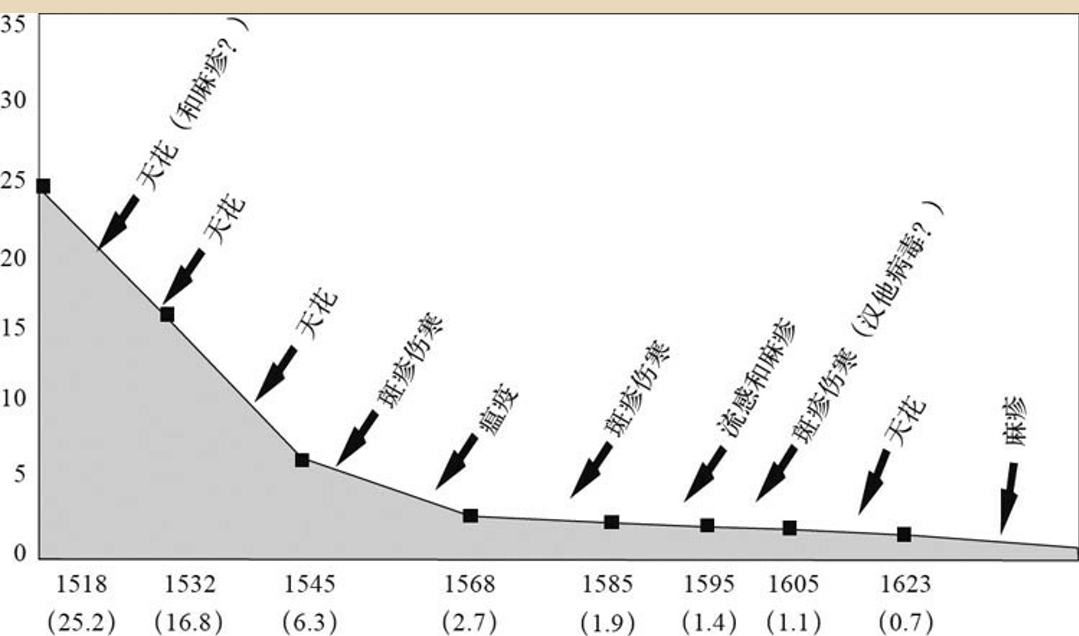
\includegraphics[width=0.7\textwidth]{images/zmzrk.jpg}
\caption{中美洲地区原著民人口变化。}
\end{figure}


总之,印第安社会的规格比人们此前相信的更大,更为古老和先进,对环境也产生过更大的影响。本书纠正了曾经风靡史学界的“霍姆伯格之误”——认为美洲大陆毫无历史和文明可言。讽刺的是,相比于气势汹汹的殖民者,印第安人表现出了巨大的包容心和道德感。墨西卡的宗教人士,甚至在和方济各修士的辩论中完全不落下风,并采用高超的修辞来表达自己的宗教信仰。

\begin{figure}[htpb]
\centering
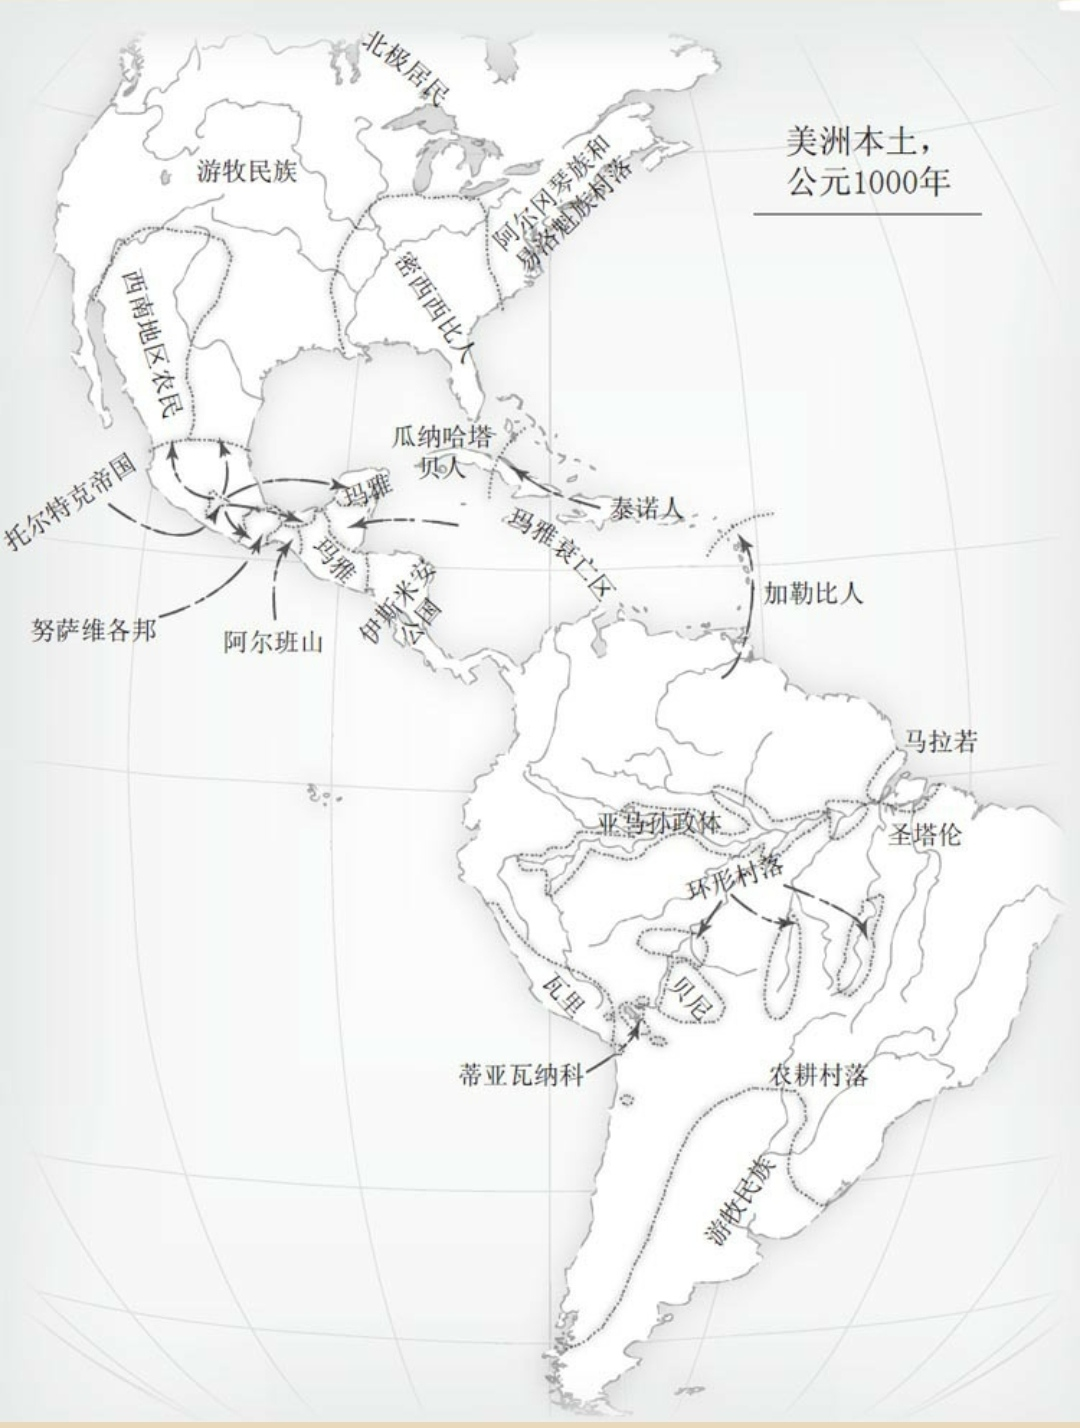
\includegraphics[width=0.5\textwidth]{images/ida-map.jpg}
\caption{美洲原著民文化分布。}
\end{figure}

印第安人在一万两千年前来到新大陆,就此就走上了与旧大陆完全不同的发展轨迹:他们独立发展出了农业,发展出了文字,发展出了国家、艺术和技术。

印第安人存在着灿烂的文明,这一点随着越来越多的考古学发现而越来越被人所知,虽然这样的发现相对于其可能出现的文明还是太少。由于与旧大陆分隔了一万多年,印第安人文明与亚欧大陆存在着巨大的差别。他们独立研究出了计数系统(绳结,包含了文字的功能)、农业(培育出影响后世的玉米、番薯、土豆等作物,中美洲驯化的作物占现在全球作物的3/5)、宗教、国家治理体系,以及天文学、独特的历法。印第安人没有与亚欧大陆的驯养动物接触过,因此无法免疫这些动物与人共同传播的一系列传染病:禽流感成为人流感、牛瘟成为麻疹、马痘成为天花。印第安人是如何培育出这些作物的?现在仍然存在很多谜团,比如玉米的野生来源是否大刍草?要知道,一般来说,由于培育者会试图除掉他们不想要的特征特性,被驯化植物的遗传多样性要小于野生物种,但玉米的多样性高于约大多数野生植物的驯化植物。

在数学上,印第安人发展出了“0”的概念,这比欧洲要先进。他们先进的数学支撑起了天文学和历法的出现。

印第安人充满了美洲的土地,相互之间存在着巨大的差异,就像中国与英国的差别那么大(甚至更大一些,毕竟亚欧大陆的文化交流在史前就已经存在了)。生机勃勃的美洲原住民文化,为这个世界提供了很多可能性,然而这种可能性随着欧洲人登陆而烟消云散。

提斯匡特姆,这个特殊的印第安人,被殖民者挟迫漂洋过海来到欧洲,在十七世纪早期代表印第安人进行了一次罕见的全球旅程。他精通西文,聪明有计谋,可谓一时的英雄豪杰。这种行为,很大程度上能够生动地表明印第安人是活生生的人,他们有着与旧大陆人的完全相同的思想、情感和毅力,并非“野蛮人”。

皮萨罗凭一人之力征服几千万人的印加帝国,很长时间内成为“文明战胜野蛮”的典范。印加人在失去自己的皇帝后如同一盘散沙,并迅速解体,成为原著民落后野蛮的注脚。然而,这件事很大程度上有着偶然性,和印加帝国的军事政治制度密切相关。历史学家多宾斯说,印加人不是被钢铁和马匹打垮的(当然也不是被火药打垮的),而是被病毒和宗派主义打垮的。

印第安人的遗传出现了巨大的同质性。在每10个美洲原住民里面,就有超过9人是O型血(几乎全体南美印第安人也都是如此),而欧洲人O型血和A型血的比例分布就平均得多。整体而言,印第安人的人类白细胞抗原种类(不超过17种)要少于欧洲(至少35种)、亚洲和非洲种群,并且数量更少;大约1/3的南美印第安人有着完全相同和近乎相同的人类白细胞抗原,非洲的数字是1/200。

印第安人虽然在生物属性上接近,但各地的文化存在着巨大的差别。其语言共有约1200种,分属多达189个语系。

印第安人并非长时间以来环保主义者认为的“生态”和“自然”,也并非环保主义的吉祥物,事实上他们大大改变了美洲的生态,现在的美洲是他们对环境的改变而形成的。比如,现在的亚马逊雨林在欧洲殖民者进入时存在着超大型的社区,而非小型渔猎社区。在亚马逊地区所有未被淹没的森林中,至少有11.9\% 的森林是“人为的”,即直接或间接地由人类活动造成的。

在本书的最后,作者更进一步,甚至认为,印第安人的生活习俗和政治传统,很大程度上影响了美国的清教徒,这对于后者建立美国政治架构有着重要作用。不过,我对这一点持保留态度。印第安人与殖民者是如何相互影响的?影响究竟有多大?这一点很难量化,似乎作者也没有给出详实的史料来佐证,而仅仅停留在猜测层面。

本书的内容十分丰富,叙述也十分精彩。作者的观察十分细腻严谨,同时他本身是反对西方中心主义的,对美洲原住民文化是喜爱和尊重的,这不同于普通的西方民众和激进的政界人士(包括政治化的环保主义者)。作者对原著民巨大的真挚的关心,融入了字里行间,读之让人警醒和反思。

评分:10/10。